\documentclass[12pt]{article}
 
\usepackage[margin=1in]{geometry}
\usepackage{amsmath,amsthm,amssymb}
\usepackage{listings}
\usepackage{graphicx}
\graphicspath{ {figures/} }
\usepackage{booktabs}
\usepackage{listings}

\newcommand{\N}{\mathbb{N}}
\newcommand{\R}{\mathbb{R}}
\newcommand{\Z}{\mathbb{Z}}
\newcommand{\Q}{\mathbb{Q}}
 
\newenvironment{theorem}[2][Theorem]{\begin{trivlist}
\item[\hskip \labelsep {\bfseries #1}\hskip \labelsep {\bfseries #2.}]}{\end{trivlist}}
\newenvironment{lemma}[2][Lemma]{\begin{trivlist}
\item[\hskip \labelsep {\bfseries #1}\hskip \labelsep {\bfseries #2.}]}{\end{trivlist}}
\newenvironment{exercise}[2][Exercise]{\begin{trivlist}
\item[\hskip \labelsep {\bfseries #1}\hskip \labelsep {\bfseries #2.}]}{\end{trivlist}}
\newenvironment{problem}[2][Problem]{\begin{trivlist}
\item[\hskip \labelsep {\bfseries #1}\hskip \labelsep {\bfseries #2.}]}{\end{trivlist}}
\newenvironment{question}[2][Question]{\begin{trivlist}
\item[\hskip \labelsep {\bfseries #1}\hskip \labelsep {\bfseries #2.}]}{\end{trivlist}}
\newenvironment{corollary}[2][Corollary]{\begin{trivlist}
\item[\hskip \labelsep {\bfseries #1}\hskip \labelsep {\bfseries #2.}]}{\end{trivlist}}
 
\begin{document}
 
\title{Homework 1}
\author{Ningyu Ma\\ 
ME614 Spring 2017}

\maketitle
Sorry for the inconvenience of the positions of figures, this is my first time using Latex so I still have not figured out how to put them into good positions.
\begin{problem}{1}
\text{}\\
$(a)$ Please see Figure 1 -12 for the log-log scale of the truncation error $\epsilon$ vs. $\Delta x^{-1}$.\\
By comparing different sets of schemes, we can find that $\epsilon_{TR}$ will decay faster with higher order of polynomial interpolant($N-1$).\\
And Staggered-Centered scheme has the fastest decay rate.\\
Note that Figure 9 should be the same as Figure 12.\\
\\
\begin{figure}[h]
\centering
  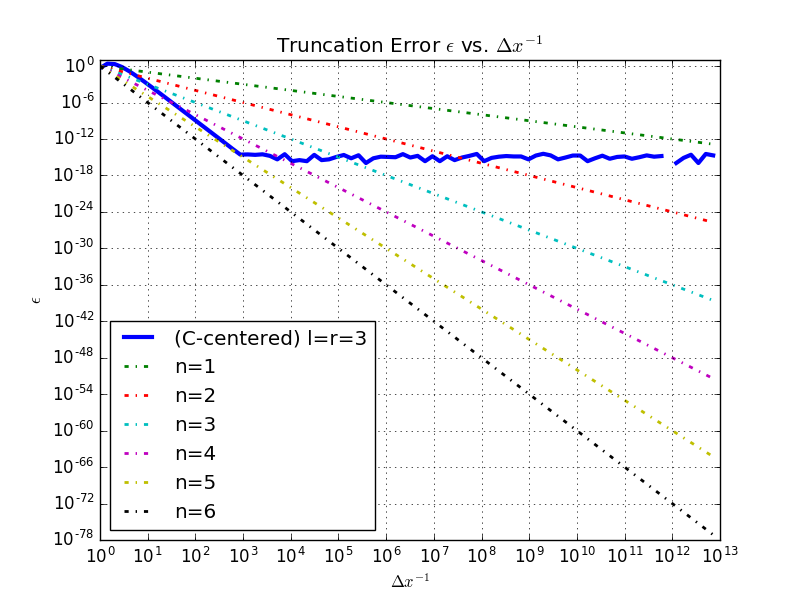
\includegraphics[scale=0.5]{ccl3r3}
 \caption{Collocated-Centered $l = r= 3$}
\label{label}
\end{figure}
\begin{figure}[h]
\centering
  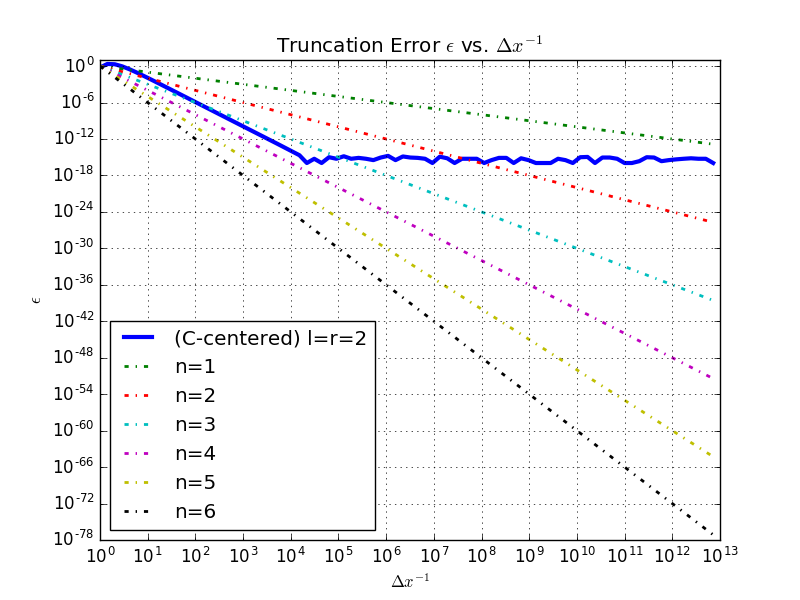
\includegraphics[scale=0.5]{ccl2r2}
 \caption{Collocated-Centered $l = r= 2$}
\label{label}
\end{figure}
\begin{figure}
\centering
  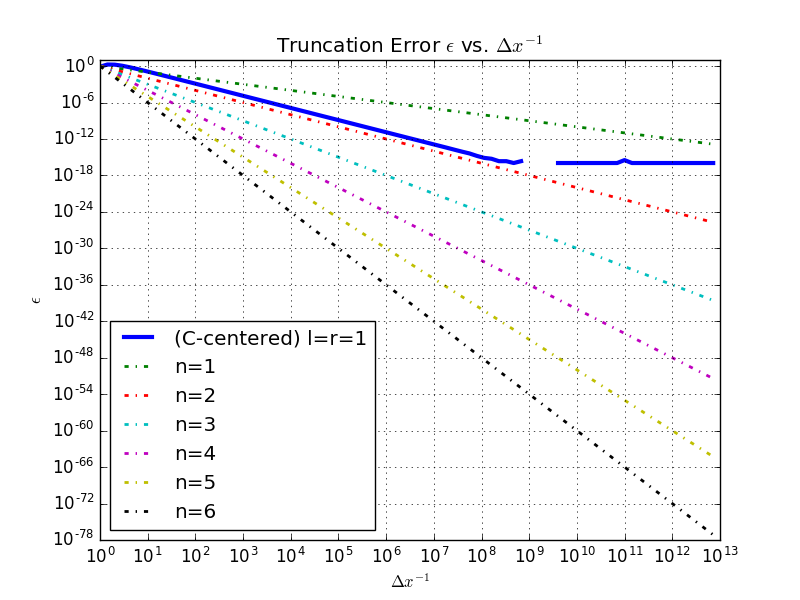
\includegraphics[scale=0.5]{ccl1r1}
 \caption{Collocated-Centered $l = r= 1$}
\label{label}
\end{figure}
\begin{figure}[h]
\centering
  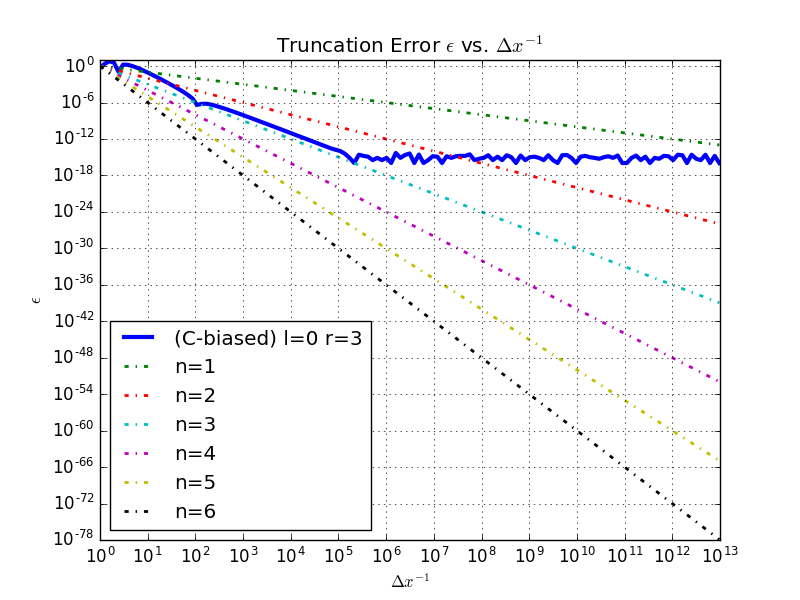
\includegraphics[scale=0.5]{cbl0r3}
 \caption{Collocated-Biased $l = 0$ $ r = 3$}
\label{label}
\end{figure}
\begin{figure}[h]
\centering
  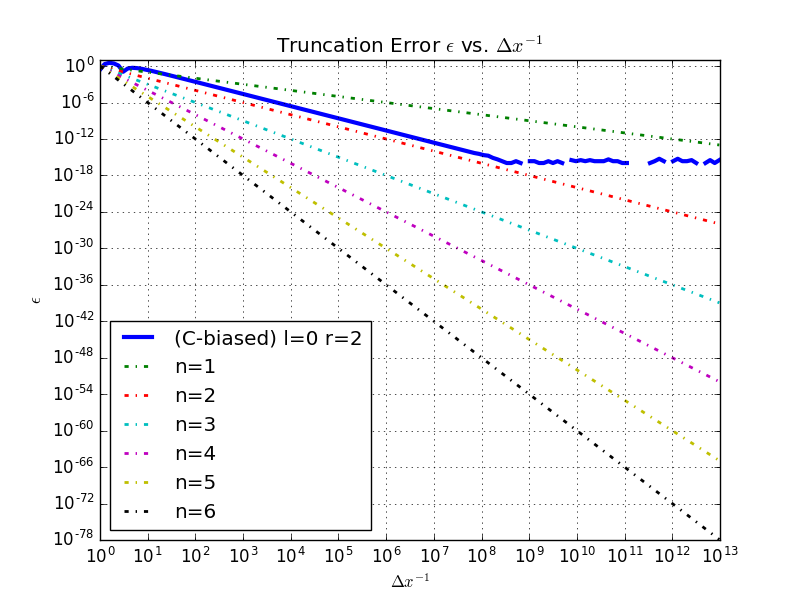
\includegraphics[scale=0.5]{cbl0r2}
 \caption{Collocated-Biased $l = 0$ $r = 2$}
\label{label}
\end{figure}
\begin{figure}
\centering
  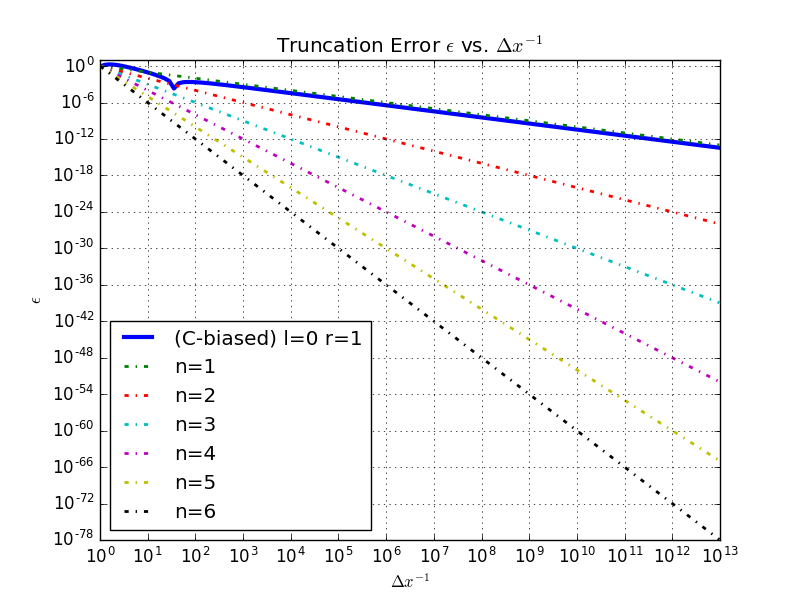
\includegraphics[scale=0.5]{cbl0r1}
 \caption{Collocated-Biased $l = 0$ $r = 1$}
\label{label}
\end{figure}
\begin{figure}
\centering
  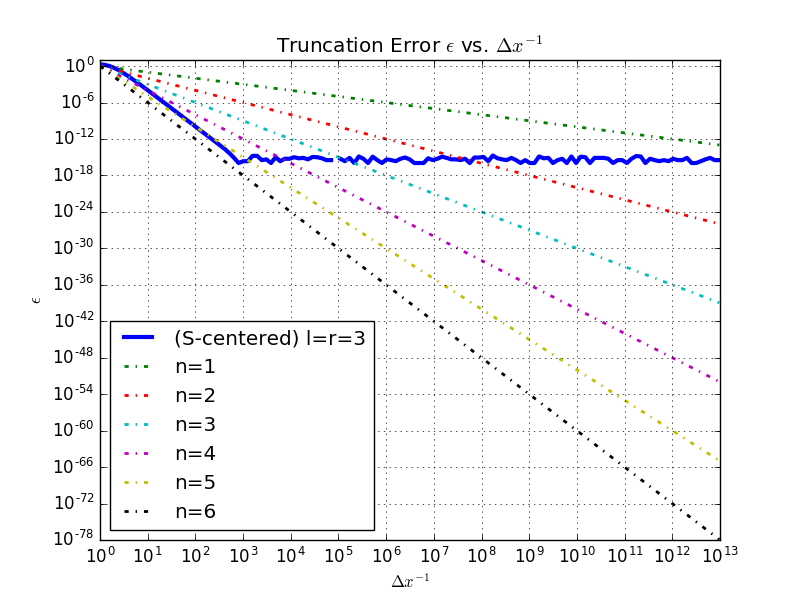
\includegraphics[scale=0.5]{scl3r3}
 \caption{Staggered-Centered $l = r= 3$}
\label{label}
\end{figure}
\begin{figure}
\centering
  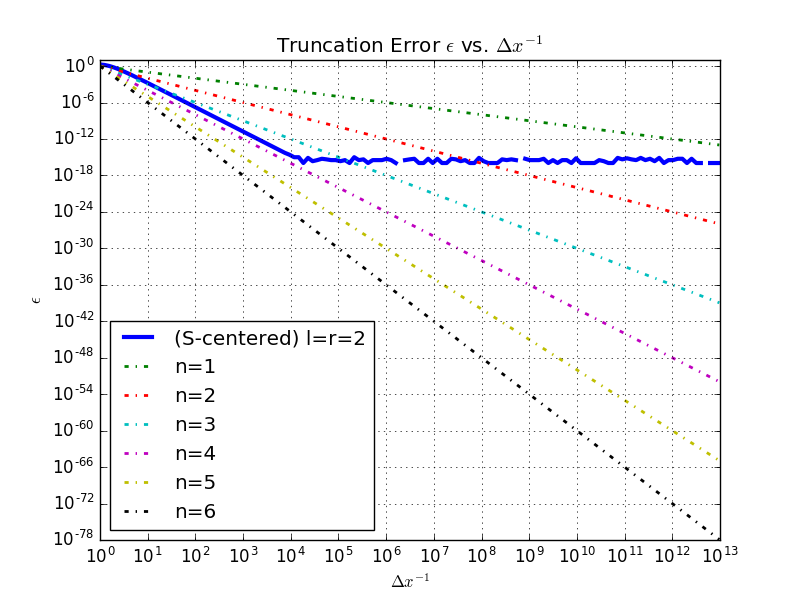
\includegraphics[scale=0.5]{scl2r2}
 \caption{Staggered-Centered $l = r= 2$}
\label{label}
\end{figure}
\begin{figure}
\centering
  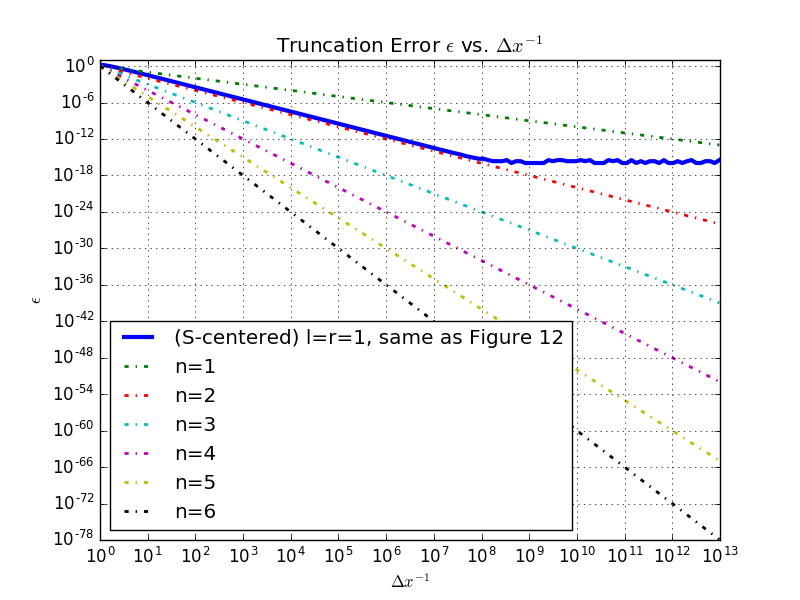
\includegraphics[scale=0.5]{scl1r1}
 \caption{Staggered-Centered $l = r= 1$}
\label{label}
\end{figure}
\begin{figure}
\centering
  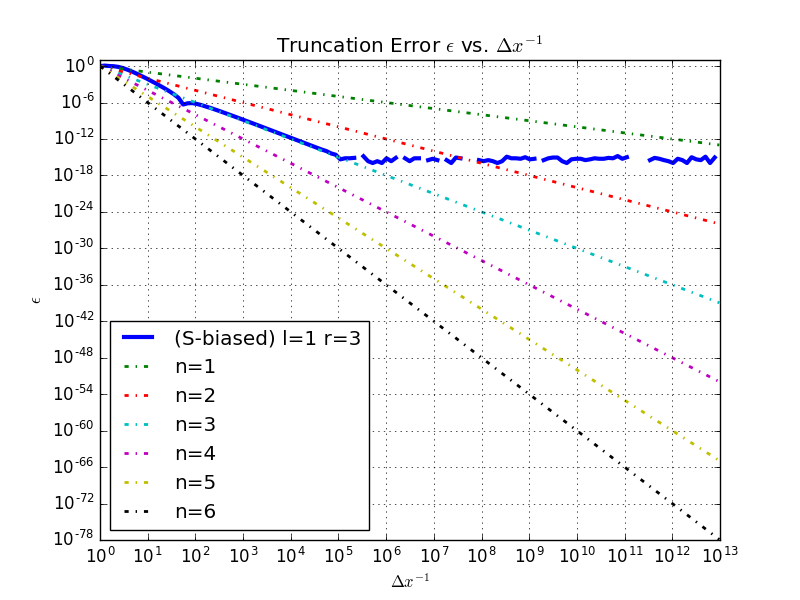
\includegraphics[scale=0.5]{sbl1r3}
 \caption{Staggered-Biased $l = 0$ $r = 3$}
\label{label}
\end{figure}
\begin{figure}
\centering
  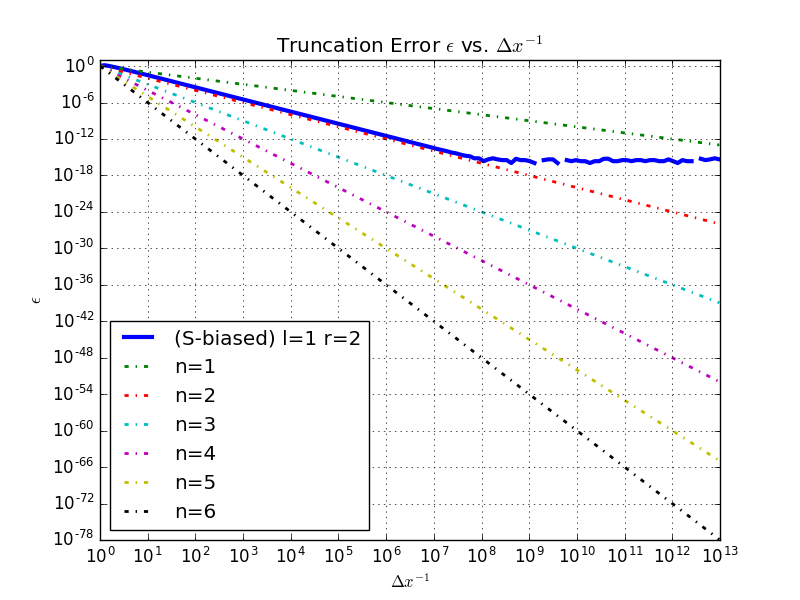
\includegraphics[scale=0.5]{sbl1r2}
 \caption{Staggered-Biased $l = 0$ $r = 2$}
\label{label}
\end{figure}
\begin{figure}
\centering
  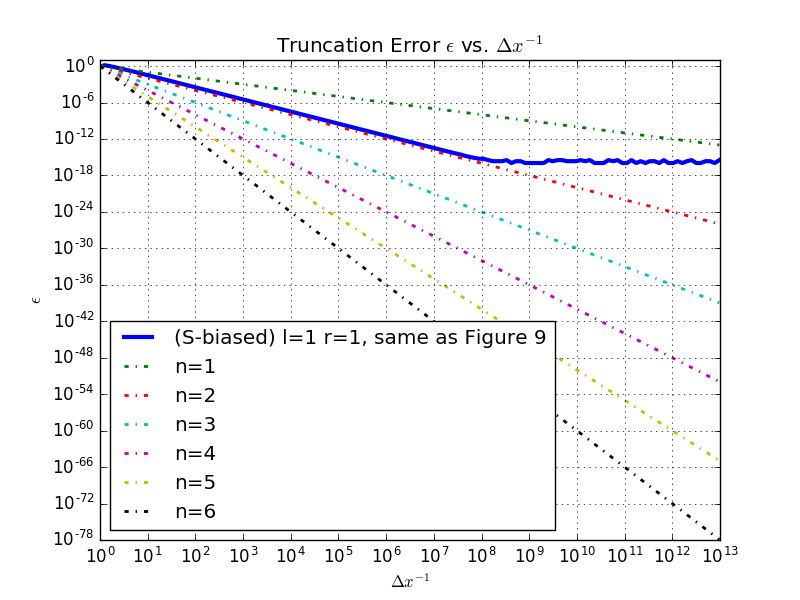
\includegraphics[scale=0.5]{sbl1r1}
 \caption{Staggered-Biased $l = 0$ $r = 1$}
\label{label}
\end{figure}
\\
$(b)$ As you can see from the plots, the order of accuracy \framebox{does not} always correspond to the order of the polynomial interpolant.\\
For a given polynomial order $p$, the minimum order of accuracy is $p$ and the maximum order of accuracy is $p+1$. But if $N$ is large enough, these two orders should be the same.\\
\end{problem}

\begin{problem}{2}
\text{ }\\
$(a)$ Please see Figure 13 - 16 for spy plots for the four schemes respectively.
\begin{figure}
\centering
  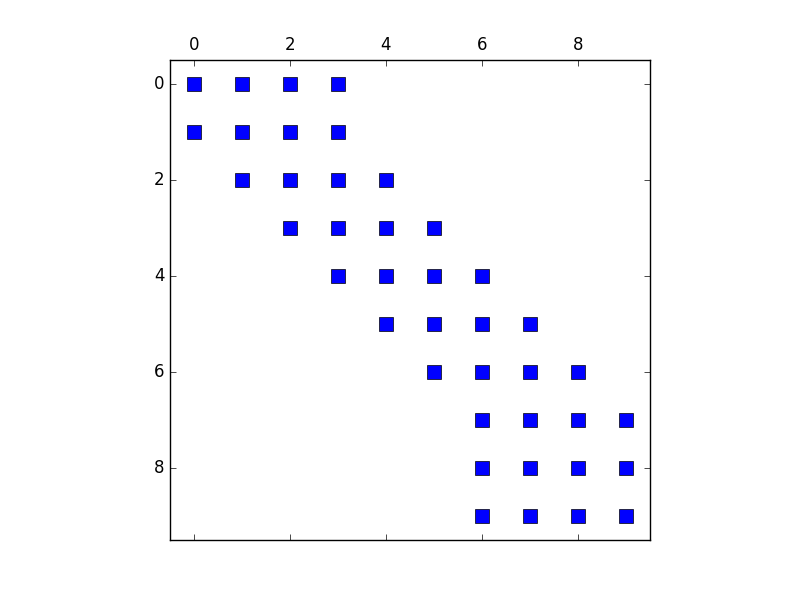
\includegraphics[scale=0.5]{p2_3p1d}
 \caption{Spy Plot of 1st-order Derivatives with 3rd-order Polynomial Reconstructions }
\label{label}
\end{figure}
\begin{figure}
\centering
  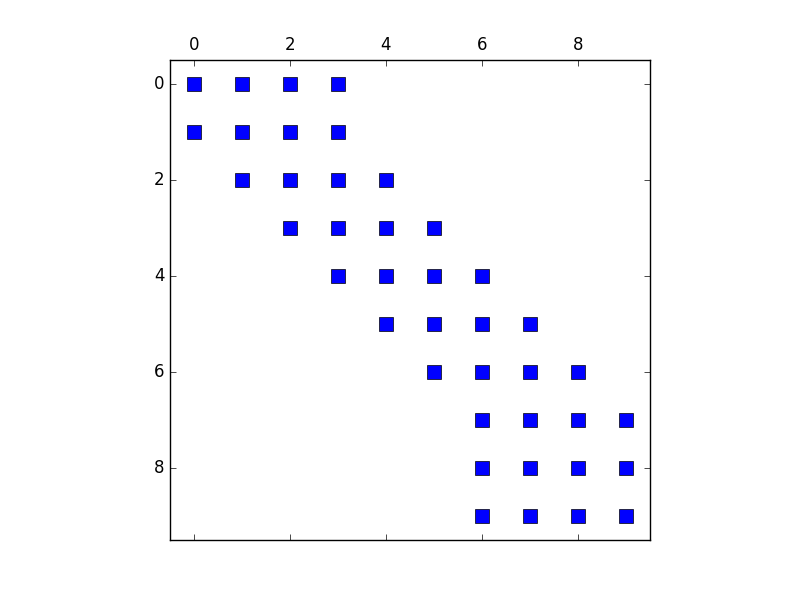
\includegraphics[scale=0.5]{p2_3p3d}
 \caption{Spy Plot of 3rd-order Derivatives with 3rd-order Polynomial Reconstructions }
\label{label}
\end{figure}
\begin{figure}
\centering
  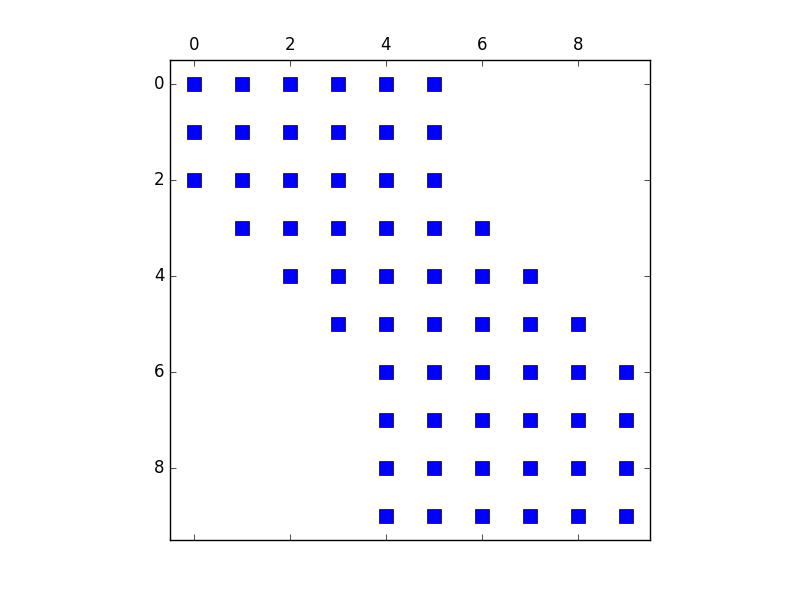
\includegraphics[scale=0.5]{p2_5p1d}
 \caption{Spy Plot of 1st-order Derivatives with 5th-order Polynomial Reconstructions }
\label{label}
\end{figure}
\begin{figure}
\centering
  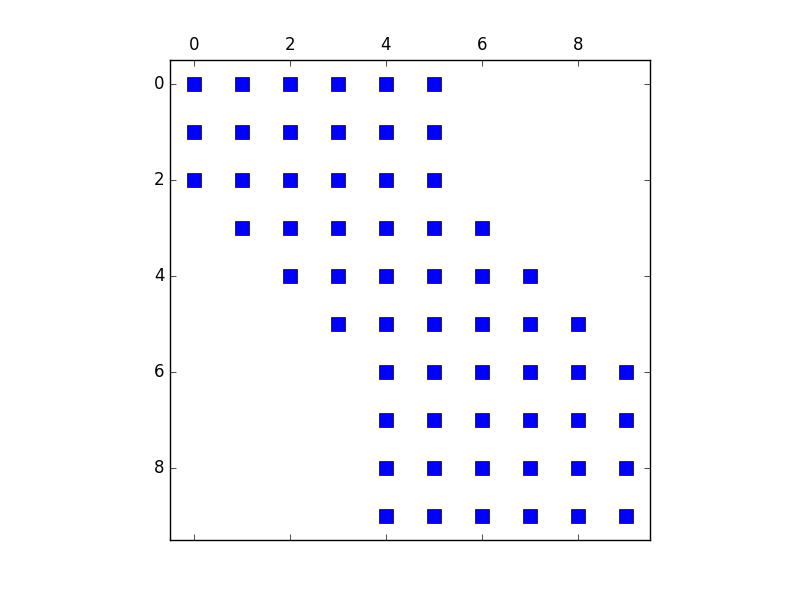
\includegraphics[scale=0.5]{p2_5p3d}
 \caption{Spy Plot of 3rd-order Derivatives with 5th-order Polynomial Reconstructions }
\label{label}
\end{figure}\\
\\
$(b)$ Please see Figure 17 - 18 for the log-log scale of the RMS vs. $\Delta x^{-1}$ of 3rd and 5th order polynomial reconstructions respectively.\\
Please noted that if I increase my iteration times of the 5th-order to 8 (I am using 7 right now), the system will produce warning: RankWarning: Polyfit may be poorly conditioned, warnings.warn(msg, RankWarning)\\
\begin{figure}
\centering
  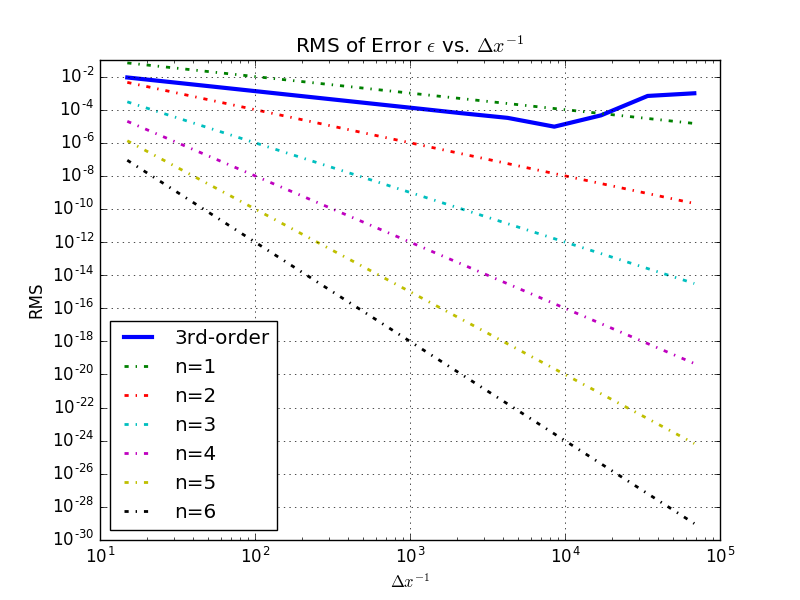
\includegraphics[scale=0.5]{p2b_3p}
 \caption{3rd-order Polynomial Reconstructions Scheme}
\label{label}
\end{figure}
\begin{figure}
\centering
  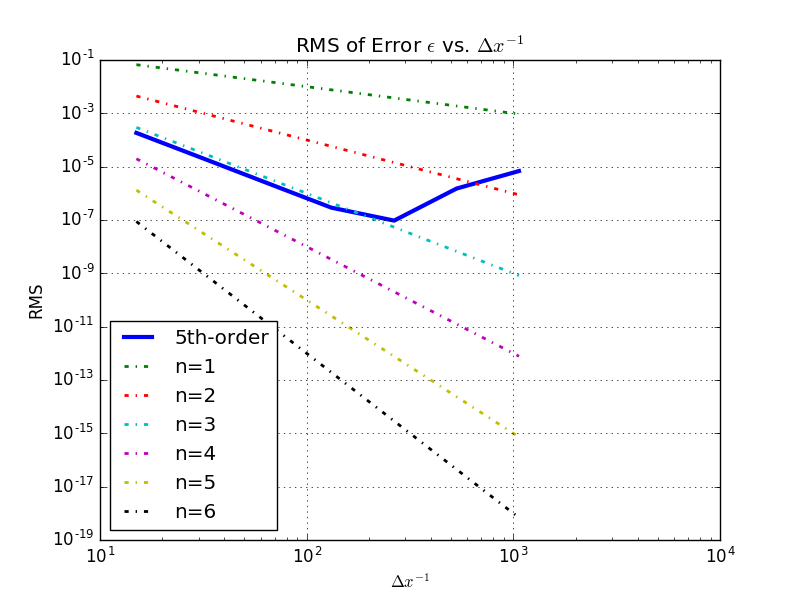
\includegraphics[scale=0.5]{p2b_5p}
 \caption{5th-order Polynomial Reconstructions Scheme}
\label{label}
\end{figure}
\end{problem}

\begin{problem}{3}
\text{ }\\ 
$(a)$ By using Pade' scheme, we need to use 5th-order Pade' scheme to derive it.\\
As illustrated in the lecture notes, we expand the derivation to 5 points:\\

\indent $\alpha_{1} \{ u_{i-2} = u_{i} - u_{i}^{(1)} \cdot  2\Delta x + u_i^{(2)} \cdot \frac{(2\Delta x)^2}{2!}  - u_i^{(3)} \cdot \frac{(2\Delta x)^3}{3!} + u_i^{(4)} \cdot \frac{(2\Delta x)^4}{4!} - u_i^{(5)} \cdot \frac{(2\Delta x)^5}{5!} + u_i^{(6)} \cdot \frac{(2\Delta x)^6}{6!}\}$\\

\indent $\alpha_{2} \{ u_{i-1} = u_{i} - u_{i}^{(1)} \cdot  \Delta x + u_i^{(2)} \cdot \frac{(\Delta x)^2}{2!} -u_i^{(3)} \cdot \frac{(\Delta x)^3}{3!} + u_i^{(4)} \cdot \frac{(\Delta x)^4}{4!} - u_i^{(5)} \cdot \frac{(2\Delta x)^5}{5!} + u_i^{(6)} \cdot \frac{(\Delta x)^6}{6!}\}$\\

\indent $\alpha_{3} \{u_{i} = u_{i} \}$\\

\indent $\alpha_{4} \{ u_{i+1} = u_{i} + u_i^{(1)} \cdot  \Delta x + u_i^{(2)} \cdot \frac{(\Delta x)^2}{2!} + u_i^{(3)} \cdot \frac{(\Delta x)^3}{3!} + u_i^{(4)} \cdot \frac{(\Delta x)^4}{4!} + u_i^{(5)} \cdot \frac{(2\Delta x)^5}{5!} + u_i^{(6)} \cdot \frac{(\Delta x)^6}{6!}\}$\\

\indent $\alpha_{5} \{ u_{i-2} = u_{i} + u_{i}^{(1)} \cdot  2\Delta x + u_i^{(2)} \cdot \frac{(2\Delta x)^2}{2!}  + u_i^{(3)} \cdot \frac{(2\Delta x)^3}{3!} + u_i^{(4)} \cdot \frac{(2\Delta x)^4}{4!} + u_i^{(5)} \cdot \frac{(2\Delta x)^5}{5!} + u_i^{(6)} \cdot \frac{(2\Delta x)^6}{6!}\}$\\

\indent $\beta_{1} \{ \Delta x^3 \cdot u_{i+1}^{(3)} = 0 + \Delta x^3 \lbrack u_{i}^{(3)} + u_{i}^{(4)} \cdot \Delta x^4 + u_i^{(5)} \cdot \frac{(\Delta x)^2}{2!} + u_i^{(6)} \cdot \frac{(\Delta x)^3}{3!} \rbrack \}$\\

\indent $\beta_{3} \{ \Delta x^3 \cdot u_{i-1}^{(3)} = 0 + \Delta x^3 \lbrack u_{i}^{(3)} - u_{i}^{(4)} \cdot \Delta x^4 + u_i^{(5)} \cdot \frac{(\Delta x)^2}{2!} - u_i^{(6)} \cdot \frac{(\Delta x)^3}{3!} \rbrack \}$\\

We multiple $\alpha_{1}$, $\alpha_{2}$, $\alpha_{3}$, $\alpha_{4}$, $\alpha_{5}$, $\beta_{1}$ and $\beta_{3}$ on both sides and add them together and, combine like terms with $u_{i}$, $u_{i}^{(1)}$, $u_{i}^{(2)}$, $u_{i}^{(3)}$, $u_{i}^{(4)}$, $u_{i}^{(5)}$ and $u_{i}^{(6)}$, we can get:\\

$\Rightarrow (\alpha_{1} + \alpha_{2} + \alpha_{3} + \alpha_{4} + \alpha_{5}) \cdot u_i\\
\indent+ (-2\alpha_{1} - \alpha_{2} + \alpha_{4} + 2\alpha_{5}) \cdot  u_{i}^{(1)}\Delta x\\
\indent+ (2\alpha_{1} + \frac{1}{2}\alpha_{2} + \frac{1}{2}\alpha_{4} + 2\alpha_{5}) \cdot  u_{i}^{(2)}\Delta x^2\\
\indent+ (-\frac{4}{3}\alpha_{1} - \frac{1}{6}\alpha_{2} + \frac{1}{6}\alpha_{4} + \frac{3}{4}\alpha_{5} + \beta_{1} + \beta_{3}) \cdot  u_{i}^{(3)}\Delta x^3\\
\indent+ (\frac{2}{3}\alpha_{1} + \frac{1}{24}\alpha_{2} + \frac{1}{24}\alpha_{4} + \frac{2}{3}\alpha_{5} + \beta_1 +\beta_3) \cdot  u_{i}^{(4)}\Delta x^4\\
\indent+ (-\frac{4}{15}\alpha_{1} + \frac{1}{120}\alpha_{2} - \frac{1}{120}\alpha_{4} + \frac{4}{15}\alpha_{5} + \frac{1}{2}\beta_{1} - \frac{1}{2}\beta_{3}) \cdot  u_{i}^{(5)}\Delta x^5\\
\indent+ (\frac{4}{45}\alpha_{1} + \frac{1}{720}\alpha_{2} + \frac{1}{720}\alpha_{4} + \frac{4}{45}\alpha_{5} + \frac{1}{6}\beta_{1} - \frac{1}{6}\beta_{3}) \cdot u_{i}^{(6)}\Delta x^6$\\
\\
Because we want to solve the 3rd-order derivative, the coefficient in front of all $u_{i}^{(m)}$ should be zero except the coefficient in front of $u_{i}^{(3)}$ is one.\\
So we have the above seven equations and seven unknowns, solve the linear system, we can got:\\
\\
\indent$\begin{cases} \alpha_1 = -1 \\ \alpha_2 = 2 \\ \alpha_3 = 0 \\ \alpha_4 = -2 \\ \alpha_5 = 1 \\ \beta_1 = -\frac{1}{2} \\ \beta_3 = \frac{1}{2} \end{cases}$\\
\\
Insert back the $\alpha$s and $\beta$s in the original equation, we can get:\\
\\
$\Rightarrow -u_{i-2} + 2u_{i-1}  -2u_{i+1} + u_{i+2} - \frac{1}{2}\Delta x^3 \cdot u_{i+1}^{(3)} + \frac{1}{2}\Delta x^3 \cdot u_{i-1}^{(3)} = \sigma(\Delta x^3)$\\
$\Rightarrow \frac{-u_{i-2} + 2u_{i-1}  -2u_{i+1} + u_{i+2}}{\Delta x^3} = \frac{1}{2}(u_{i+1}^{(3)} - u_{i-1}^{(3)})$\\
\\
So the order of accuracy is 3.\\
\\
I do not have time but I think I know the basic concept for the rest of problem 3.\\
$\Rightarrow$\\
Then we can write the above equation in a form of:\\
$\Rightarrow \underline{L}$ $\underline{\hat{u^{(3)}}}$ $=$ $\underline{R}$ $\underline{U}$\\
$\Rightarrow \underline{\hat{u^{(3)}}}$ $=$ $\underline{L^{-1}}$ $\underline{R}$  $\underline{U}$\\
$\Rightarrow \underline{\hat{u^{(3)}}}$ $=$ $\underline{D}$ $\underline{U}$\\
Where $\underline{D}$ should be a full rank matrix.\\
\\
Also, we have to insert the three boundary conditions in the first, second last and last row of matrix $\underline{D}$ like Problem $2(b)$ and use the linear solver to get $\underline{\hat{u^{(3)}}}$ at the end.\\

\end{problem}





\end{document}
